\begin{frame}
  \frametitle{Smooth Maps Between Manifolds}
  \begin{defn}
    A smooth manifold $M$ of dimension $n$ is a 
    topological manifold of dimension $n$
    together with a maximal smooth atlas 
    $\{(U_\alpha, \phi_\alpha)\}$.
  \end{defn}
  \begin{center}
    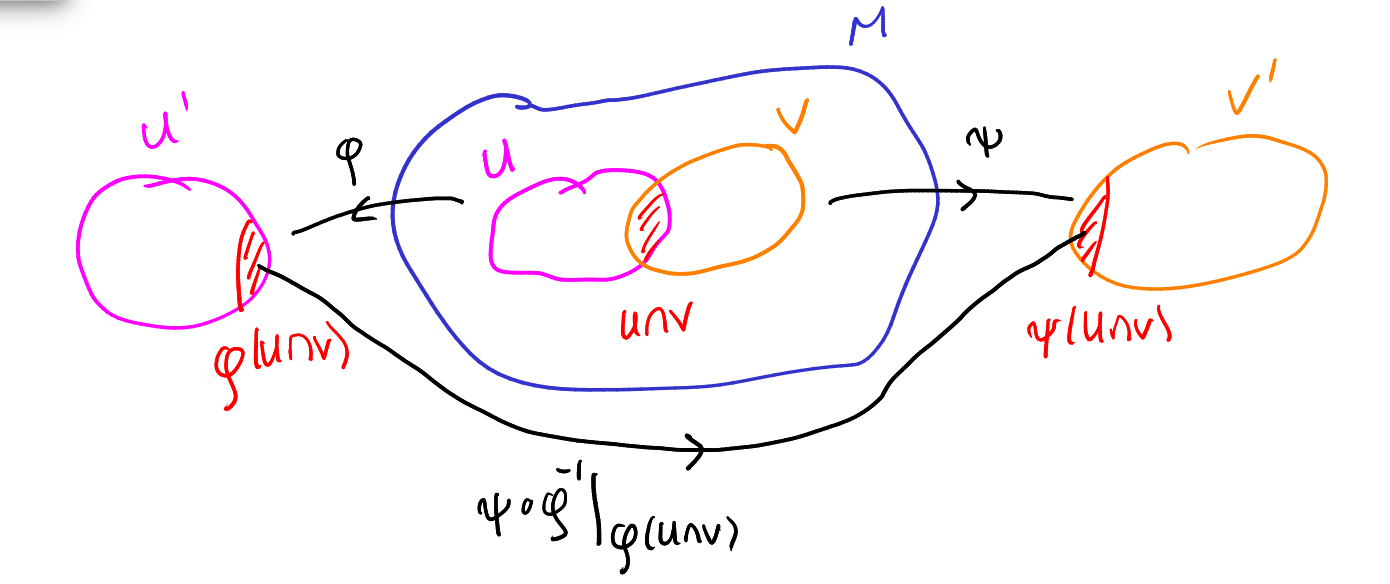
\includegraphics[width=0.5\textwidth]{figures/two_charts.png}
  \end{center}
  \begin{defn}
    A continuous function $f \colon M \to \R^m$ is
    smooth at $p \in M$ if for every chart $(U, \phi)$
    with $p \in U$, the map
    $f \circ \phi^{-1} \colon \phi(U) \to \R^m$
    is smooth at $\phi(p)$.

    The function $f$ is smooth on $M$ if it is smooth at every 
    $p \in M$.
  \end{defn}
\end{frame}
\begin{frame}
  \begin{prop}
    The following are equivalent:
    \begin{enumerate}[(i)]
      \item $f \colon M \to \R^m$ is smooth
      \item $M$ has an atlas such that
        for every chart $(U_\alpha, \phi_\alpha)$ in the atlas,
        $f \circ \phi_\alpha^{-1}$ is smooth.
      \item For every chart $(V, \psi)$ on $M$ the 
        function $f \circ \psi^{-1}$ is smooth.
    \end{enumerate}
  \end{prop}
  \begin{proof}
    By definintion (i) and (iii) are equivalent.
    We show that (ii) implies (iii) and that (iii) implies (ii).
    Clearly (iii) implies (ii), so we only need to show
    that (ii) implies (iii).
    Let $\{(U_\alpha, \phi_\alpha)\}$ be a smooth atlas for the
    differentiable structure on $M$ and let $(U, \phi)$ be a 
    chart on $M$. Let $p \in U$ and pick a chart $(U_\alpha, \phi_\alpha)$
    in the given atlas
    with $p \in U_\alpha$. 
    By (ii), the map $f \circ \phi_\alpha^{-1}$ is smooth. Restricted to
    $\phi(U \cap U_\alpha)$ we have
    \begin{displaymath}
      f \circ \phi^{-1} = (f \circ \phi_\alpha^{-1}) \circ
      (\phi_\alpha \circ \phi^{-1})
    \end{displaymath}
    This is a composition of two smooth maps between open 
    sets in Euclidean space, so it is smooth at $\phi(p)$.
  \end{proof}
\end{frame}
\begin{frame}
  \begin{example}
    The inclusion $S^1 \subseteq \R^2$ is smooth.
    We can see this by considering the atlas we constructed earlier where
    one of the charts $(U, \phi)$ given as
    \begin{displaymath}
      U = \{(x,y) \in S^1 \cond x > 0\}, \quad \phi \colon U \to (-1,1),
      \quad \phi(x, y) = y.
    \end{displaymath}
    Then $\phi^{-1}(t) = (\sqrt{1 - t^2}, t)$ is smooth. 

    Similarly for the other charts.
  \end{example}
\end{frame}
\begin{frame}
  \begin{block}
    {Observation}
    A map $f \colon M \to \R^m$ is smooth if and only if 
    the map $f \circ \phi^{-1}$ is smooth.
  \end{block}
  \begin{defn}
    Let $M$ and $N$ be smooth manifolds with $\dim(M) = m$ and
    $\dim(N) = n$. A continuous map $F \colon N \to M$ is {\em smooth}
    at a point $p \in N$ for every chart $(V, \psi)$ about $F(p)$ 
    in $M$, the map $\psi \circ F \colon F^{-1}(V) \to \R^m$
    is smooth at $p$.
    The map $F$ is {\em smooth} if it is smooth at every $p \in N$.
  \end{defn}
  \begin{remark}
    Since $F^{-1}(V)$ is an open subset of $N$, it is a smooth mainfold of 
    dimension $n$.
  \end{remark}
  \begin{remark}
    $F$ is smooth if and only if for all charts $(U, \phi)$ for $N$ and 
    all charts $(V, \psi)$ for $M$, the composed map 
    $\phi^{-1} \circ F \circ \psi \colon \phi(U) \to \R^m$ is smooth.
  \end{remark}
\end{frame}
\begin{frame}
  \begin{remark}
    Considering $M = \R^n$ as a smooth mainfold with the standard
    differential structure, by the previous proposition,
    a map $F \colon N \to M$ is a smooth map of manifolds 
    if and only if the map $F \colon N \to \R^n$ is smooth
    in the sense introduced first.
  \end{remark}
\end{frame}
\begin{frame}
  \begin{prop}
    The following are equivalent:
    \begin{enumerate}[(i)]
      \item $F \colon N \to M$ is smooth
      \item There exists an atlas $\{(V_\beta, \psi_\beta)\}$
        for $M$ such that for every chart $(V_\beta, \psi_\beta)$
        in the atlas, the map $\psi_\beta \circ F \colon F^{-1}(V) \to \R^m$
        is smooth.
      \item For every chart $(V, \psi)$ on $M$ the map
        $\psi \circ F \colon F^{-1}(V) \to \R^m$ is smooth.
    \end{enumerate}
  \end{prop}
  \begin{proof}
    Again, we only need to show that (ii) implies (iii).
    Let $(U, \psi)$ be a chart on $M$. We need to show that 
    for every $p \in N$ with $F(p) \in U$, the map $\psi \circ F$ is smooth
    at $p$. Pick a chart $(V_\beta, \psi_\beta)$ with $F(p) \in V_\beta$.
    Then restricted to $F^{-1}(V \cap V_{\beta})$ we have
    \begin{displaymath}
      \psi \circ F = (\psi \circ \psi_{\beta}^{-1}) \circ (\psi_\beta \circ F).
    \end{displaymath}
    Since $\psi_\beta \circ F$ is smooth at $p$ and
    $\psi \circ \psi_{\beta}^{-1} \colon \psi_{\beta}(V \cap V_{\beta}) \to \psi(V)$
    is smooth, we conclude that 
    $\psi \circ F$ is smooth at $p$.
  \end{proof}
\end{frame}
\begin{frame}
  \begin{prop}
    If $F \colon N \to M$ and $G \colon M \to P$
    are smooth maps of smooth manifolds, then so is 
    the composite $G \circ F \colon N \to P$.
  \end{prop}
  \begin{proof}
    Let $p \in N$, let $(V, \psi)$ be a chart around $F(p) \in M$ 
    and let $(W, \sigma)$ be a chart around $G \circ F(p)$ in $P$.
    Then locally,
    \begin{displaymath}
      \sigma \circ (G \circ F) = (\sigma \circ G \circ \psi^{-1}) \circ (\psi
      \circ F)
    \end{displaymath}
    is a composition of smooth maps between open subsets of Euclidean space.
  \end{proof}
  \begin{example}
    Suppose that $f \colon \R^2 \to \R$ is smooth.

    Then the restriction to $i \colon S^1 \to \R^2$ of
    $f$ is a smooth map $f \vert_{S^1} \colon S^1 \to \R$.
    This is because that $f \vert_{S^1}  = f \circ i$
    is the composition of two smooth maps.
  \end{example}
\end{frame}
\begin{frame}
  \begin{defn}
    A smooth map $f \colon N \to M$ is a {\em diffeomorphism} if there
    exists a smooth map $g \colon M \to N$ such that $g$ is inverse to $f$,
    that is, such that $g \circ f = \id_N$ and $f \circ g = \id_M$.
  \end{defn}
  \begin{example}
    Every chart $(U, \phi)$ for $M$ is a diffeomorphism
    \begin{displaymath}
      \phi \colon U \to \phi(U) \subseteq \R^n.
    \end{displaymath}
    Thus, a smooth $n$-dimensional manifold is locally 
    diffeomorphic to an open subset of $\R^n$.
  \end{example}
  \begin{thm}[Stalling $\sim 1960$]
    If $n \ne 4$, then any two smooth structures on $\R^n$ are
    diffeomorphic.
  \end{thm}
  \begin{thm}[Donaldson $\sim 1980$]
    There exists a smooth structure on $\R^4$ which is not 
    diffeomorphic to the standard smooth structure.
  \end{thm}
\end{frame}
\begin{frame}
  Let $M$ be an $n$-dimensional smooth manifold and let $(U, \phi)$ 
  be a chart on $M$. Let $r^1, \dots, r^n$ be the standard coordinates
  on $\R^n$ and write $x^i = r^i \circ \phi \colon U \to \R$.
  Then $\phi(p) = (x^1(p), \dots, x^n(p))$. We write $(U, x^1, \dots, x^n)$
  for this chart.
  \begin{center}
    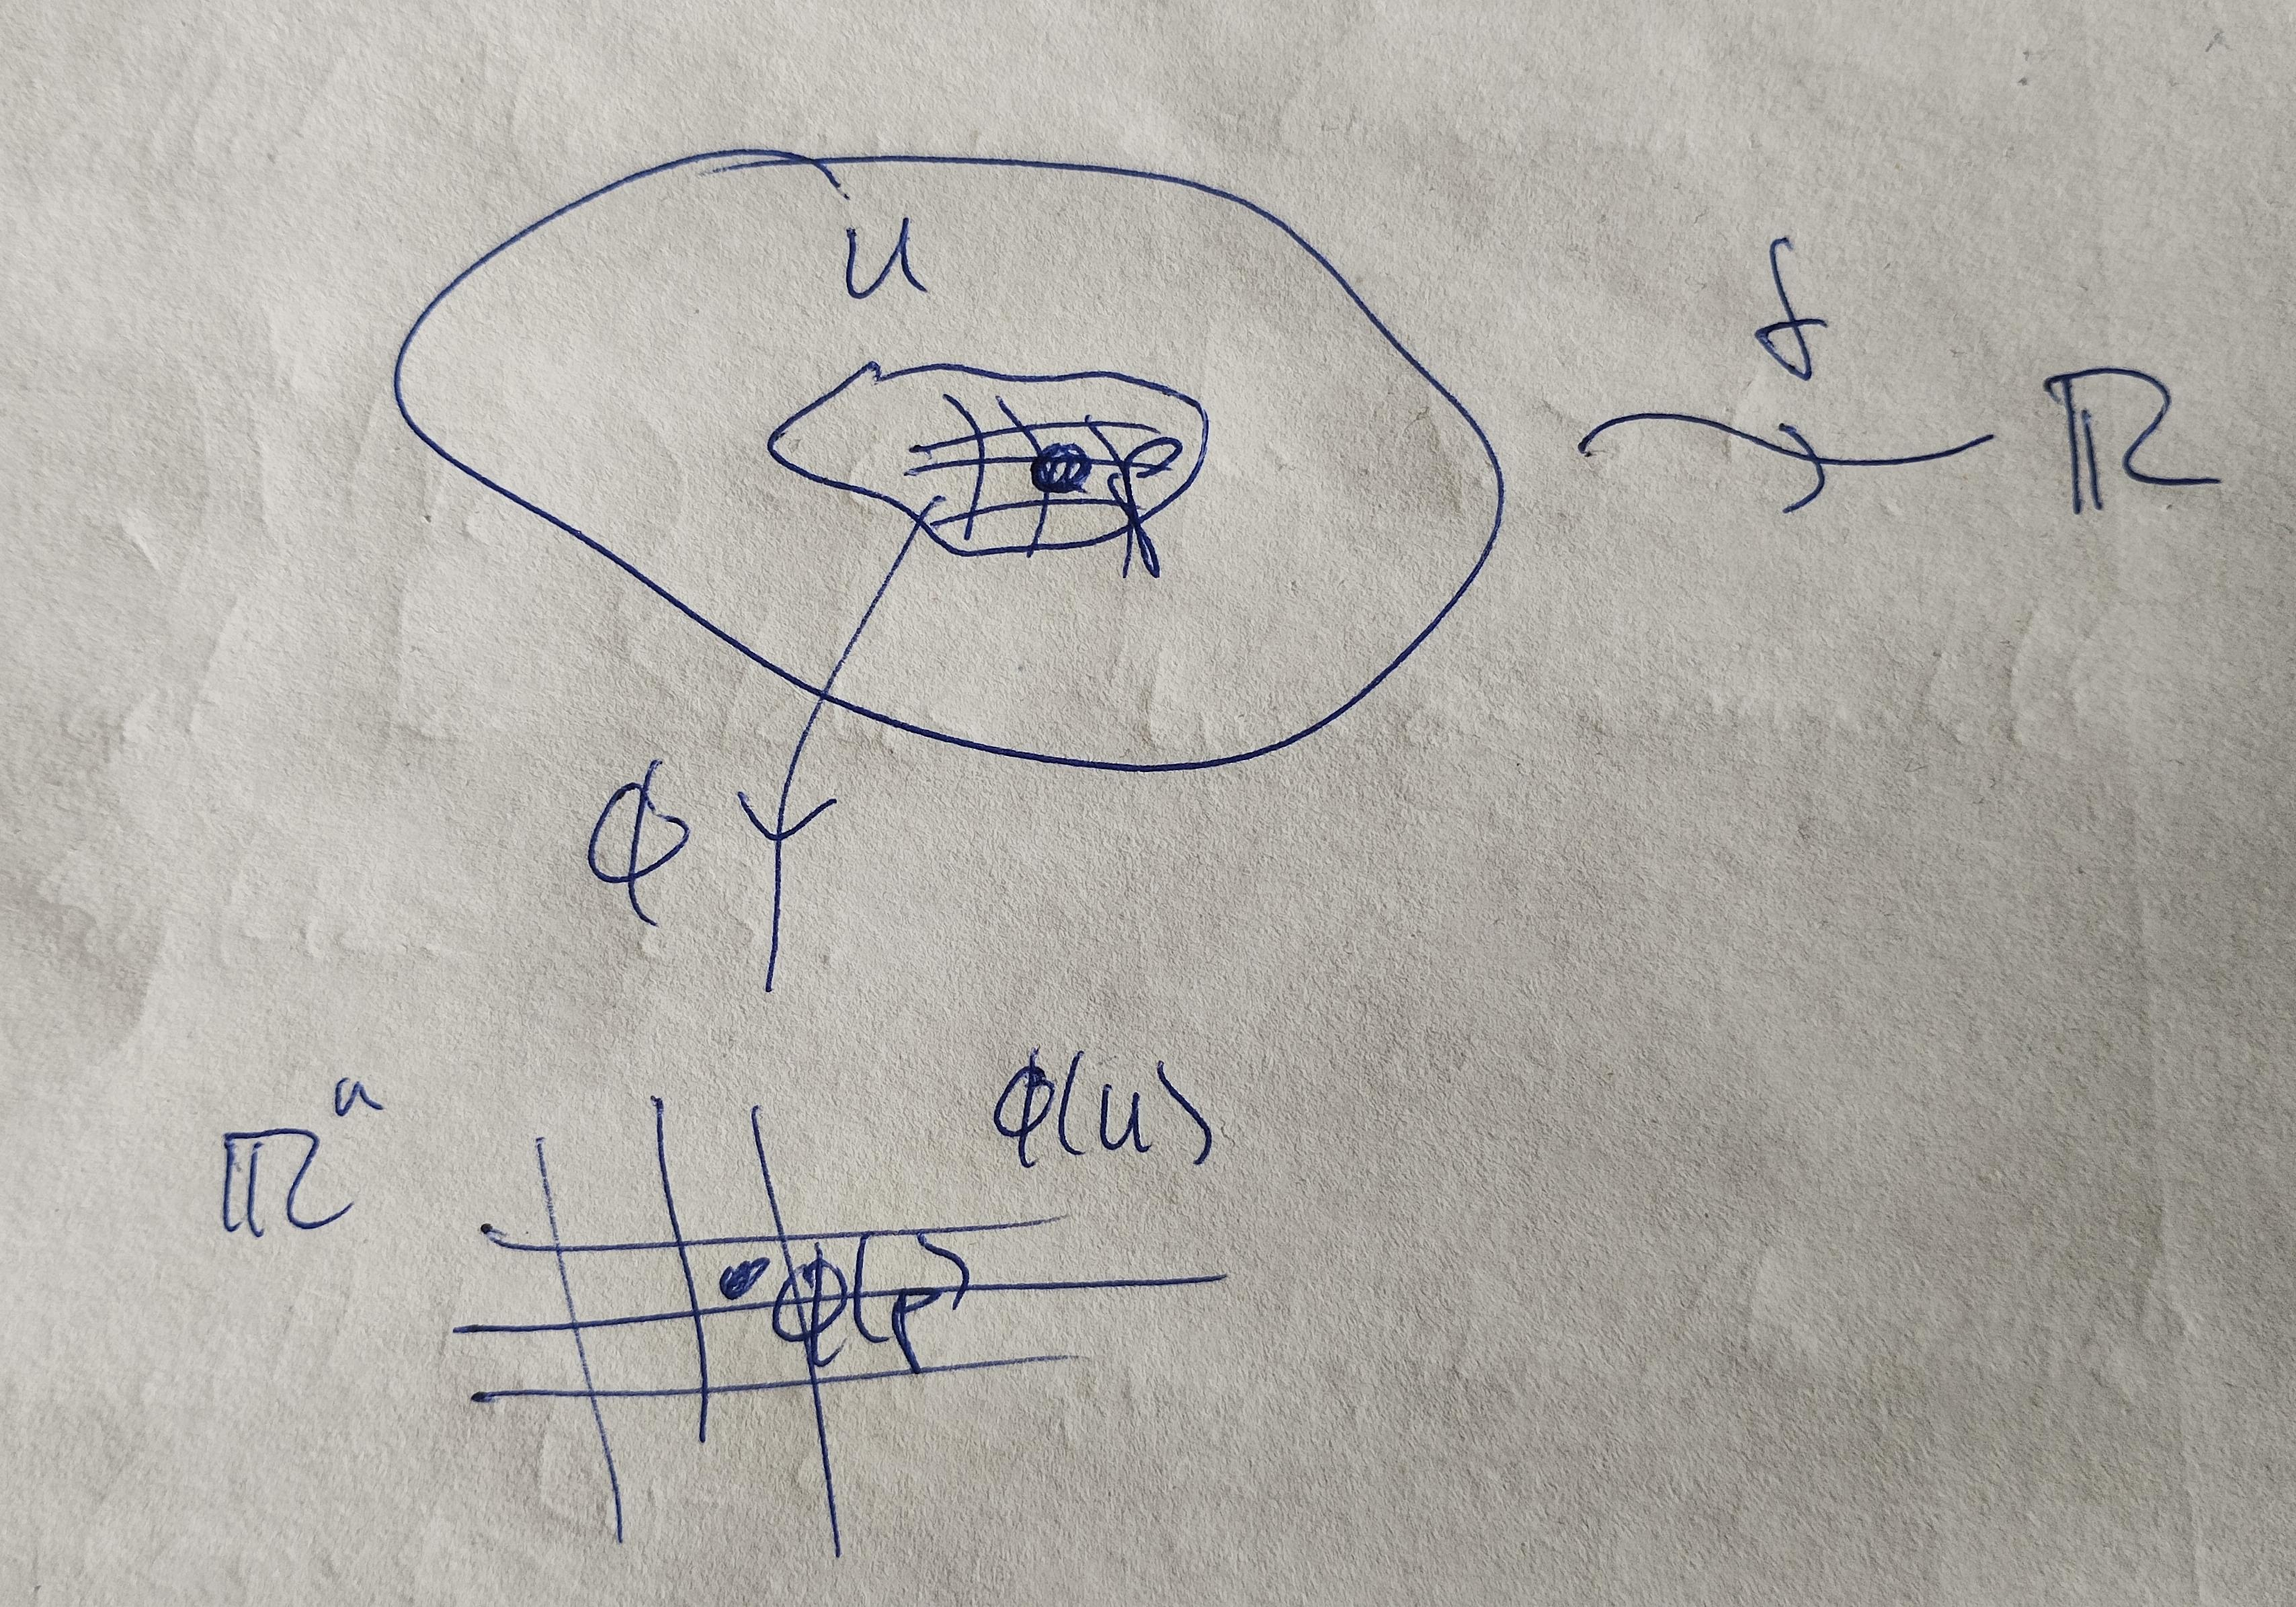
\includegraphics[width=0.3\textwidth]{figures/coordinates.jpg}
  \end{center}
  \begin{defn}
    Let $f \colon M \to \R$ be a smooth map. The local partial derivatives
    of $f$ with respect to the chart $(U, x^1, \dots, x^n)$ at $p \in U$
    are
    \begin{displaymath}
      \frac{\partial f}{\partial x^i}(p) = \frac{\partial f \circ \phi^{-1}}
      {\partial r^i}(\phi(p))
    \end{displaymath}
  \end{defn}
\end{frame}
\begin{frame}
  Notice that 
  the function
  \begin{displaymath}
    \frac{\partial f}{\partial x^i}= \frac{\partial f \circ \phi^{-1}}
    {\partial r^i} \circ \phi \colon U \to \R
  \end{displaymath}
  is smooth.
  For $f = x^i$ we get 
  \begin{displaymath}
    \frac{\partial x^i}{\partial x^j}(p)= \delta^j_i.
  \end{displaymath}
  Given a smooth map $F \colon N \to M$, choose a chart
  $(U, \phi) = (U, x^1, \dots, x^n)$ for $N$ and a chart
  $(V, \psi) = (V, y^1, \dots, y^m)$ for $M$ such that $F(U) \subseteq V$.
  Let $F^i = y^i \circ F \colon U \to \R$.
  \begin{defn}
    The {\em Jacobian } of $F$ at $p \in U$ with respect to $(U, \phi)$
    and $(V, \psi)$ is the matrix
    \begin{displaymath}
      \left[\frac{\partial F^i}{\partial x^j}(p)\right] = 
      \left[\frac{\partial y^i \circ F \circ \phi^{-1}}{\partial r^j}(\phi(p))\right]
    \end{displaymath}
  \end{defn}
\end{frame}
\begin{frame}
  Observe that if $U = N = \R^n$ and $V = M = \R^m$ 
  with their standard coordinates, then we recover the Jacobian
  from calculus.
  \begin{example}
    If $F = \id_N$, then this is the usual Jacobian of the transition 
    function $\psi \circ \phi^{-1}$. More precisely, it is easy to verify that
    \begin{displaymath}
      \frac{\partial({\psi \circ \phi^{-1}})^i}{\partial r^j}(\phi(p)) =
      \frac{\partial y^i}{\partial x^j}(p).
    \end{displaymath}
  \end{example}
\end{frame}
\begin{frame}
  \frametitle{The Inverse Function Theorem}
  \begin{defn}
    A smooth function $F \colon M \to N$ is a {\em local diffeomorphism}
    at a point $p \in M$ if there exists a neighborhood $U$ of $p$
    such that $F\vert_U \colon U \to F(U) \subseteq N$ is a
    diffeomorphism to an open set $F(U)$ in $N$.
  \end{defn}
  \begin{example}
    $f(x) = x^2$ is a local diffeomorphism at $x = 1 \in \R$ but not at $x = 0$.
  \end{example}
\end{frame}
\begin{frame}
  % \frametitle{Inverse Function Theorem for $\R^n$}
  \begin{thm}[Inverse Function Theorem for $\R^n$]
    Let $U \subseteq \R^n$ be open. 
    A smooth map $F \colon U \to \R^n$ is a local diffeomorphism
    at $p \in U$ if and only if the Jacobian
    \begin{displaymath}
      \left[
        \frac{\partial F^i}{\partial r^j}(p)
      \right]
    \end{displaymath}
    is invertible.
  \end{thm}
  \begin{thm}[Inverse Function Theorem for smooth manifolds]
    Let $N$ and $M$ be smooth manifolds of dimension $n$ and let
    $F \colon N \to M$ be a smooth map. Given $p \in N$, choose 
    charts $(U, x^1, \dots, x^n)$ about $p$ in $N$ and 
    $(V, y^1, \dots, y^n)$ for $M$ such that $F(U) \subseteq V$.
    Then $F$ is a local diffeomorphism
    at $p \in U$ if and only if the Jacobian
    \begin{displaymath}
      \left[
        \frac{\partial F^i}{\partial x^j}(p)
      \right]
    \end{displaymath}
    is invertible.
  \end{thm}
\end{frame}
\begin{frame}
  \begin{proof}
    \begin{center}
      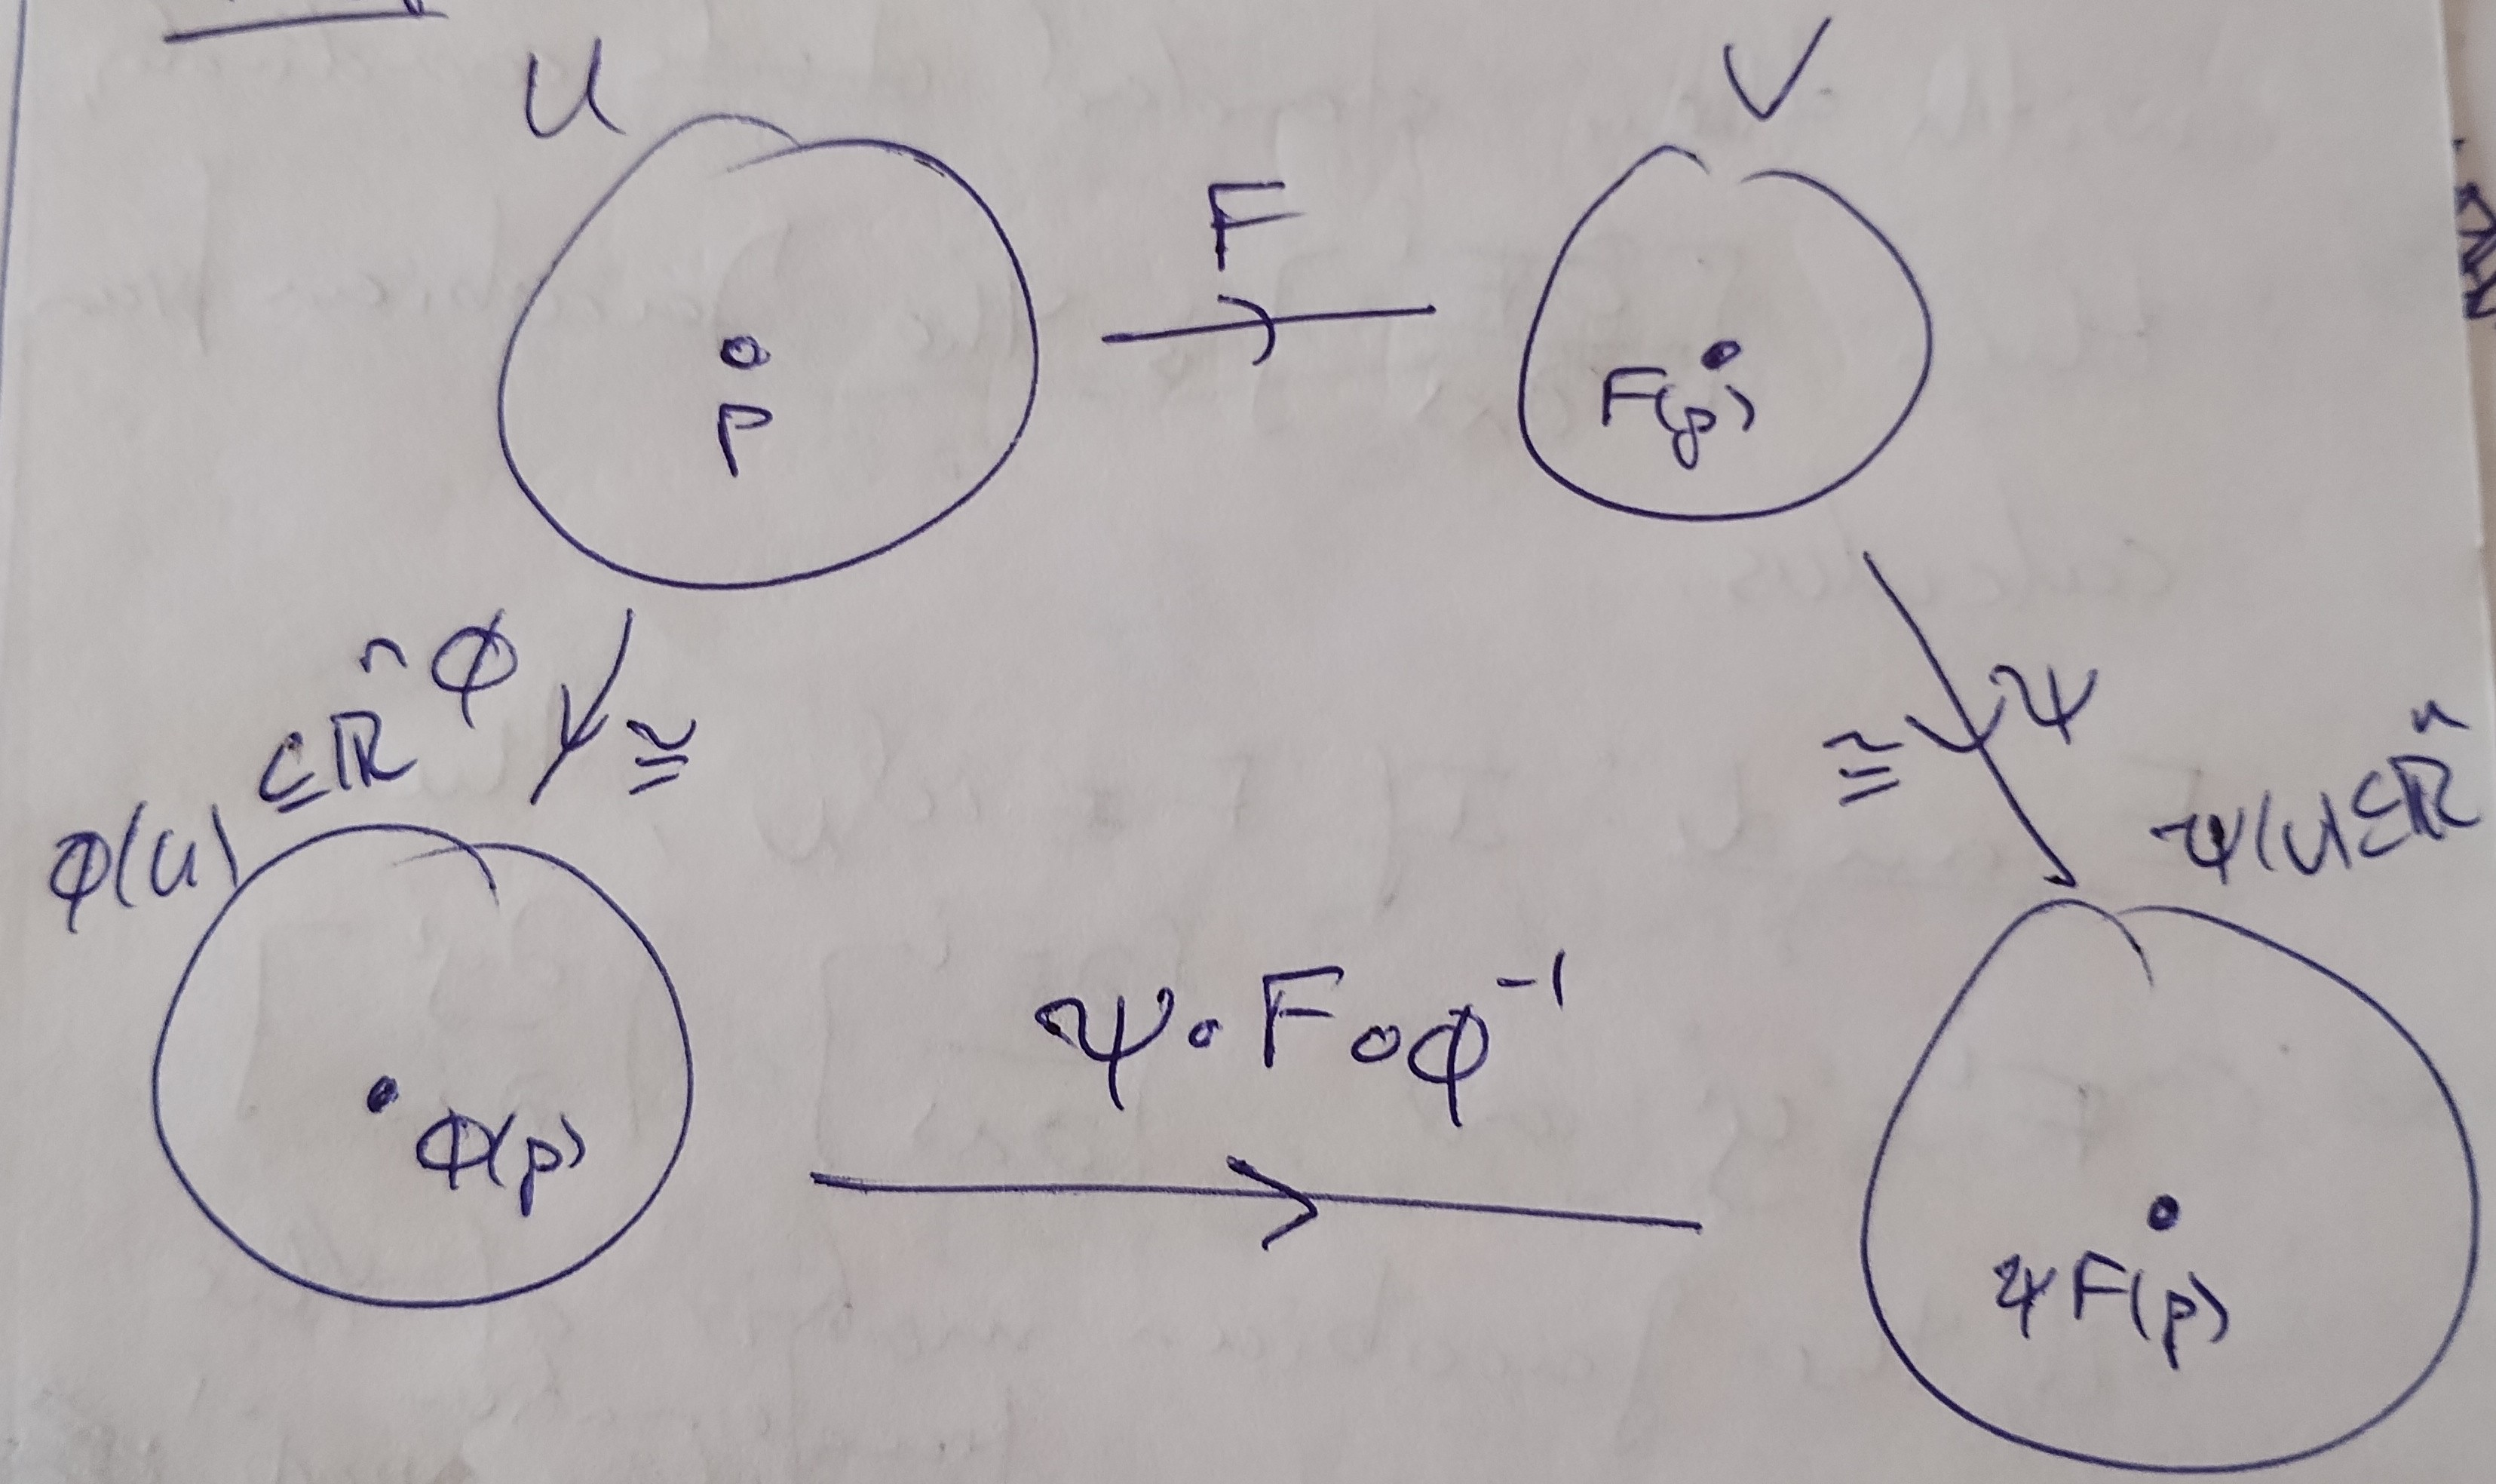
\includegraphics[width=0.4\textwidth]{figures/coordinate_change.jpg}
    \end{center}
    We know from the inverse function theorem for $\R^n$ that 
    the matrix
    $
      \left[
        \frac{\partial r^i \circ (\psi \circ F \circ \phi^{-1})}{\partial
        r^j}(\phi(p))
      \right]
    $
    is invertible if and only if $\psi \circ F \circ \phi^{-1}$ 
    is a local diffeomorphism at $\phi(p)$. By the above illustration 
    this is the case if and only if $F$ is a local diffeomorphism at $p$.
    However,
    \begin{displaymath}
      \left[
        \frac{\partial F^i}{\partial x^j}(p) 
        \right]
      =
      \left[
        \frac{\partial (r^i \circ \psi \circ F)}{\partial x^j}(p) 
        \right]
      =
      \left[
        \frac{\partial (r^i \circ \psi \circ F)}{\partial x^j}(p) 
        \right]
      =
      \left[
        \frac{\partial (r^i \circ \psi \circ F \phi^{-1})}{\partial
        r^j}(\phi(p))
        \right]
    \end{displaymath}
  \end{proof}
\end{frame}
\begin{frame}
  \frametitle{Lie Groups}
  \begin{defn}
    A {\em Lie group} is a smooth manifold $G$
    with smooth maps
    \begin{displaymath}
      \mu \colon G \times G \to G \quad \text{and}
      \quad \iota \colon G \to G
    \end{displaymath}
    such that the product $xy = \mu(x, y)$ and inverse $x^{-1} = \iota (x)$
    form a group structure on $G$.
  \end{defn}
  \begin{example}
    \begin{enumerate}[(i)]
      \item $\R^n$ with addition 
      \item $\C^\times = \C \setminus \{0\}$ with multiplication
      \item $S^1$ with complex multiplication
      \item The general linear group $GL(n, \R)$ of invertible 
        $n \times n$-matrices with matrix multiplication. In fact, 
        $GL(n, \R)$ can be veiwed as an open subset of $\R^{n^2}$.
    \end{enumerate}
  \end{example}
\end{frame}
